\section{Other Features} %Local Invariant Reasoning, Register Recycling, If-Closure and Address Calculation}
\label{sec:complications}

\subsection{Local Invariant Reasoning ($\xLIR$)}
\label{sec:tc1}

\begin{example}
  \label{ex:tc1}
  JMM causality Test Case 1 \citep{PughWebsite} states the following
  execution should be allowed ``since interthread compiler analysis could
  determine that $x$ and $y$ are always non-negative, allowing simplification
  of $r{\geq}0$ to true, and allowing write $y\GETS1$ to be moved early.''
  \begin{gather*}
    x\GETS 0 \SEMI
    \FORK{\!
      (r\GETS x\SEMI\IF{r{\geq}0}\THEN y\GETS1 \FI
      \PAR
      x\GETS y)
    }
    \\[-1ex]
    \hbox{\begin{tikzinline}[node distance=1.5em]
        \event{wx0}{\DW{x}{0}}{}
        \event{rx1}{\DR{x}{1}}{right=3em of wx0}
        \event{wy1}{1{\geq}1\mid\DW{y}{1}}{right=of rx1}
        \event{ry1}{\DR{y}{1}}{right=3em of wy1}
        \event{wx1}{\DW{x}{1}}{right=of ry1}
        \po{ry1}{wx1}
        \rf[out=-168,in=-12]{wx1}{rx1}
        \rf{wy1}{ry1}
        \wk[out=10,in=170]{wx0}{wx1}
        \wk{wx0}{rx1}
        \po{rx1}{wy1}
      \end{tikzinline}}
  \end{gather*}
  Under the definitions given thus far, the precondition on $\DWP{y}{1}$ can
  only be satisfied by the read of $x$, disallowing this execution.

  In order to allow such executions, we include memory references in formula,
  resulting in:
  \begin{gather*}
    % x\GETS 0 \SEMI
    % \FORK{\!
    % (r\GETS x\SEMI\IF{r{\geq}0}\THEN y\GETS1 \FI
    % \PAR
    % x\GETS y)
    % }
    %   \\[-1ex]
    \hbox{\begin{tikzinline}[node distance=1.5em]
        \event{wx0}{\DW{x}{0}}{}
        \event{rx1}{\DR{x}{1}}{right=3em of wx0}
        \event{wy1}{0{\geq}0\mid\DW{y}{1}}{right=of rx1}
        \event{ry1}{\DR{y}{1}}{right=3em of wy1}
        \event{wx1}{\DW{x}{1}}{right=of ry1}
        \po{ry1}{wx1}
        \rf[out=-168,in=-12]{wx1}{rx1}
        \rf{wy1}{ry1}
        \wk[out=10,in=170]{wx0}{wx1}
        \wk{wx0}{rx1}
      \end{tikzinline}}
  \end{gather*}
\end{example}

% In order to allow such executions, we include memory references in formula.
% (\ref{L4} is unchanged in \refdef{def:pomsets-lir}.)

\begin{definition}[\xLIR]
  \label{def:pomsets-lir}
  Update \refdef{def:pomsets-trans} to (\ref{L4} unchanged):
  \begin{enumerate}
  \item[{\labeltext[S4]{S4)}{S4}}]
    $\aTr{\bEvs}{\bForm}$ implies $\bForm[\aExp/\aLoc]$,
  \item[{\labeltext[S5]{S5)}{S5}}]
    $\aTr{\cEvs}{\bForm}$ implies $\bForm[\aExp/\aLoc]$,
  \item[{\labeltext[L4]{L4)}{L4}}]
    $\aTr{\bEvs}{\bForm}$ implies $\aVal{=}\aReg\limplies\bForm$, 
  \item[{\labeltext[L5]{L5)}{L5}}]
    $\aTr{\cEvs}{\bForm}$ implies
    $(\aVal{=}\aReg\lor\aLoc{=}\aReg)\limplies\bForm$, when $\aEvs\neq\emptyset$,
  \item[{\labeltext[L6]{L6)}{L6}}] 
    $\aTr{\dEvs}{\bForm}\;$ implies $\bForm$, $\aEvs=\emptyset$.
  \end{enumerate}
\end{definition}

\ref{L5} introduces memory references.  It states that to be independent of
the read, we establish both $\bForm[\aVal/\aReg]$ and $\bForm[\aLoc/\aReg]$.
If a precondition holds in both circumstances, \ref{S5} allows a local write
to satisfy the precondition without introducing dependence.

One reading of \ref{L5} is that when satisfying a precondition $\aForm$ it is
safe to ignore a read as long as $\aForm$ is compatible with both the value
of the read and the value of the preceding local write.  This begs the
question: what value must $\aForm$ be compatible with in the case that the
pomset is empty?  In this case, there is no value $\aVal$ to check!
Therefore the best we can do is to emulate skip, as in \ref{L6}.  In order to
eventually arrive at a top-level pomset, this means that subsequent code must
be independent of $\aReg$.

\begin{example}
  Revisiting \refex{ex:tc1} and eliding irrelevant transformers:
  \begin{align*}
    \begin{gathered}[t]
      \PW{x}{0} 
      \\
      \hbox{\begin{tikzinline}[node distance=.5em and 1.5em]
          \event{a0}{\DW{x}{0}}{}
          \xform{xi}{\bForm[0/x]}{below=of a0}
        \end{tikzinline}}    
    \end{gathered}
    &&
    \begin{gathered}[t]
      \PR{x}{r} 
      \\
      \hbox{\begin{tikzinline}[node distance=.5em and 1.5em]
          \event{a1}{\DR{x}{1}}{}
          \xform{xi}{(1{=}r\lor x{=}r)\limplies\bForm}{below=of a1}
        \end{tikzinline}}    
    \end{gathered}
    &&
    \begin{gathered}[t]
      \IF{r{\geq}0}\THEN y\GETS1 \FI
      \\
      \hbox{\begin{tikzinline}[node distance=.5em and 1.5em]
          \event{a2}{r{\geq}0\mid\DW{y}{1}}{}      
        \end{tikzinline}}    
    \end{gathered}
  \end{align*}
  Composing:
  \begin{align*}
    \begin{gathered}[t]
      \PW{x}{0} 
      \SEMI\PR{x}{r} 
      \SEMI\IF{r{\geq}0}\THEN y\GETS1 \FI
      \\
      \hbox{\begin{tikzinline}[node distance=.5em and 1.5em]
          \event{a0}{\DW{x}{0}}{}
          \event{a1}{\DR{x}{1}}{right=of a0}
          \event{a2}{(1{=}r\lor 0{=}r)\limplies r{\geq}0\mid\DW{y}{1}}{right=of a1}      
        \end{tikzinline}}    
    \end{gathered}
  \end{align*}
  The precondition of $\DWP{y}{1}$ is a tautology, as required.
\end{example}

\subsection{Register Recycling ($\xRecycle$)}

The semantics considered thus far assume that each register is assigned at
most once in a program.  We relax this by renaming.
\begin{example}
  \label{ex:tc2}
  JMM causality Test Case 2 \citep{PughWebsite} states the following
  execution should be allowed ``since redundant read elimination could result
  in simplification of $\aReg{=}\bReg$ to true, allowing $y\GETS1$ to be
  moved early.''
  \begin{gather*}
    \PR{x}{r}\SEMI
    \PR{x}{s}\SEMI
    \IF{r{=}s}\THEN \PW{y}{1}\FI
    \PAR
    x\GETS y
    \\
    \hbox{\begin{tikzinline}[node distance=1.5em]
        \event{a1}{\DR{x}{1}}{}
        % \event{a2}{\DR{x}{1}}{right=of a1}
        \event{a3}{\DW{y}{1}}{right=of a1}
        \po{a1}{a3}
        % \po[out=-20,in=-160]{a1}{a3}
        \event{b1}{\DR{y}{1}}{right=3em of a3}
        \event{b2}{\DW{x}{1}}{right=of b1}
        \rf{a3}{b1}
        \po{b1}{b2}
        % \rf[out=169,in=11]{b2}{a2}
        \rf[out=169,in=11]{b2}{a1}
      \end{tikzinline}}
  \end{gather*}
  This execution is not allowed under \refdef{def:pomsets-lir}, since the
  precondition of $\DWP{y}{1}$ in the independent case is
  \begin{displaymath}
    (r{=}1 \lor r{=}x)\limplies (s{=}1 \lor s{=}r)\limplies (r{=}s),
  \end{displaymath}
  which is not a tautology.  Our solution is to rename registers using the
  set $\uRegs{\AllEvents}=\{\uReg{\aEv}\mid\aEv\in\AllEvents\}$, which are
  banned from source programs, as per \textsection\ref{sec:prelim}.  This
  allows us to resolve nondeterminism in loads when merging, resulting in:
  \begin{gather*}
    \hbox{\begin{tikzinline}[node distance=1.5em]
        \event{a1}{\DR{x}{1}}{}
        % \event{a2}{\DR{x}{1}}{right=of a1}
        \event{a3}{\DW{y}{1}}{right=of a1}
        % \po{a1}{a3}
        % \po[out=-20,in=-160]{a1}{a3}
        \event{b1}{\DR{y}{1}}{right=3em of a3}
        \event{b2}{\DW{x}{1}}{right=of b1}
        \rf{a3}{b1}
        \po{b1}{b2}
        % \rf[out=169,in=11]{b2}{a2}
        \rf[out=169,in=11]{b2}{a1}
      \end{tikzinline}}
  \end{gather*}
\end{example}


\begin{definition}[$\xRecycle$]
  \label{def:pomsets-if}
  Update \refdef{def:pomsets-trans} to:
  \begin{enumerate}
  \item[\ref{L4})] 
    $\aTr{\bEvs}{\bForm}$ implies $\aVal{=}\uReg{\aEv}\limplies\bForm[\uReg{\aEv}/\aReg]$, 
  \item[\ref{L5})] 
    % $\aTr{\cEvs}{\bForm}$ implies $(\aVal_\aEv{=}\uReg{\aEv}\lor \aLoc{=}\uReg{\aEv})\allowbreak\limplies\bForm[\uReg{\aEv}/\aReg]$,
    % \item[\ref{L6})] 
    $(\forall\bReg)$ $\aTr{\cEvs}{\bForm}$ implies $\bForm[\bReg/\aReg]$. 
  \end{enumerate}
\end{definition}

\begin{example}
  Revisiting \refex{ex:tc2}, eliding irrelevant transformers and choosing
  $\uReg{\aEv}=r$:
  \begin{align*}
    \begin{gathered}[t]
      \PR{x}{r} 
      \\
      \hbox{\begin{tikzinline}[node distance=.5em and 1.5em]
          \eventl{e}{a0}{\DR{x}{0}}{}
          \xform{xi}{(1{=}r\lor x{=}r)\limplies\bForm[r/r]}{below=of a0}
        \end{tikzinline}}    
    \end{gathered}
    &&
    \begin{gathered}[t]
      \PR{x}{s} 
      \\
      \hbox{\begin{tikzinline}[node distance=.5em and 1.5em]
          \eventl{e}{a1}{\DR{x}{1}}{}
          \xform{xi}{(1{=}r\lor x{=}r)\limplies\bForm[r/s]}{below=of a1}
        \end{tikzinline}}    
    \end{gathered}
    % &&
    % \begin{gathered}[t]
    %   \IF{r{\geq}s}\THEN y\GETS1 \FI
    %   \\
    %   \hbox{\begin{tikzinline}[node distance=.5em and 1.5em]
    %     \event{a2}{r{=}s\mid\DW{y}{1}}{}      
    %   \end{tikzinline}}    
    % \end{gathered}
  \end{align*}
  Coalescing and composing:
  \begin{align*}
    \begin{gathered}[t]
      \PR{x}{r}
      \SEMI
      \PR{x}{s}
      \\
      \hbox{\begin{tikzinline}[node distance=.5em and 1.5em]
          \eventl{e}{a0}{\DR{x}{0}}{}
          \xform{xi}{(1{=}r\lor x{=}r)\limplies\bForm[r/s]}{below=of a0}
        \end{tikzinline}}    
    \end{gathered}
    &&
    \begin{gathered}[t]
      \IF{r{\geq}s}\THEN y\GETS1 \FI
      \\
      \hbox{\begin{tikzinline}[node distance=.5em and 1.5em]
          \event{a2}{r{=}s\mid\DW{y}{1}}{}      
        \end{tikzinline}}    
    \end{gathered}
  \end{align*}
  Composing:
  \begin{align*}
    \begin{gathered}[t]
      \PR{x}{r}
      \SEMI
      \PR{x}{s}
      \SEMI
      \IF{r{\geq}s}\THEN y\GETS1 \FI
      \\
      \hbox{\begin{tikzinline}[node distance=.5em and 1.5em]
          \eventl{e}{a0}{\DR{x}{0}}{}
          \event{a2}{(1{=}r\lor x{=}r)\limplies r{=}r\mid\DW{y}{1}}{right=of a0}      
        \end{tikzinline}}    
    \end{gathered}
  \end{align*}
  The precondition of $\DWP{y}{1}$ is a tautology, as required.
\end{example}


\subsection{If-Closure ($\xIF$)}
\label{sec:if}

% x+0 = x
% if (y==0) { x+y 

% Requires indexing to resolve nondeterminism.

% IF closure/case analysis: $\psi_e$

\begin{example}
  \label{ex:if1}
  If $\aCmd=(\PW{x}{1})$, then \refdef{def:pomsets-trans} does \emph{not} allow:
  \begin{gather*}
    \IF{\aExp}\THEN\PW{x}{1}\FI
    \SEMI
    \aCmd
    \SEMI
    \IF{\lnot\aExp}\THEN\PW{x}{1}\FI
    \\
    \hbox{\begin{tikzinline}[node distance=1em]
        \event{a}{\DW{x}{1}}{}
        \event{b}{\DW{x}{1}}{right=of a}
        \wk{a}{b}
      \end{tikzinline}}
  \end{gather*}
  However, if
  $\aCmd=(\IF{\lnot\aExp}\THEN\PW{x}{1}\FI\SEMI\IF{\aExp}\THEN\PW{x}{1}\FI)$,
  then it %\refdef{def:pomsets-trans}
  \emph{does} allow the execution.  Looking at the initial program:
  \begin{align*}
    \begin{gathered}
      \IF{\aExp}\THEN\PW{x}{1}\FI
      \\
      \hbox{\begin{tikzinline}[node distance=1em]
          \event{a}{\aExp\mid\DW{x}{1}}{}
        \end{tikzinline}}
    \end{gathered}
    &&
    \begin{gathered}
      \PW{x}{1}
      \\
      \hbox{\begin{tikzinline}[node distance=1em]
          \event{a}{\DW{x}{1}}{}
        \end{tikzinline}}
    \end{gathered}
    &&
    \begin{gathered}
      \IF{\lnot\aExp}\THEN\PW{x}{1}\FI
      \\
      \hbox{\begin{tikzinline}[node distance=1em]
          \event{a}{\lnot\aExp\mid\DW{x}{1}}{}
        \end{tikzinline}}
    \end{gathered}
  \end{align*}
  \noindent
  The difficulty is that the middle action can coalesce either with the right
  action, or the left, but not both.  Thus, we are stuck with some
  non-tautological precondition.  Our solution is to allow a pomset to
  contain many events for a single action, as long as the events have
  disjoint preconditions.

  This is not simply a theoretical question; it is observable.
  \refdef{def:pomsets-trans} does not allow the following.
  \begin{gather*}
    \begin{gathered}
      \PR{y}{r}\SEMI
      \IF{r}\THEN\PW{x}{1}\FI \SEMI
      \PW{x}{1} \SEMI
      \IF{\lnot r}\THEN\PW{x}{1}\FI\SEMI
      \PW{z}{r}
      \\[-.5ex]{}\PAR{}
      \IF{x}\THEN
        \PW{x}{0} \SEMI
        \IF{x}\THEN \PW{y}{1} \FI
      \FI
    \end{gathered}    
    \\
    \hbox{\begin{tikzinline}[node distance=1em]
        \event{a1}{\DW{x}{1}}{}
        \event{a2}{\DW{x}{1}}{right=of a1}
        \wk{a1}{a2}
        \event{a0}{\DR{y}{1}}{left=of a1}
        \event{a3}{\DW{z}{1}}{right=of a2}
        \po[out=20,in=160]{a0}{a3}
        \event{b0}{\DR{x}{1}}{below right=1em and -1em of a0}
        \event{b1}{\DW{x}{0}}{right=of b0}
        \event{b2}{\DR{x}{1}}{right=of b1}
        \event{b3}{\DW{y}{1}}{right=of b2}
        \wk{b0}{b1}
        \wk{b1}{b2}
        \po{b2}{b3}
        \rf{b3}{a0}
        \rf{a1}{b0}
        \rf{a2}{b2}
        \wk{b1}{a2}
      \end{tikzinline}}
  \end{gather*}  
\end{example}
% \begin{example}
%   \label{ex:if1}
%   \refdef{def:pomsets-trans} does \emph{not} allow:
%   \begin{gather*}
%     \aCmd=\PBR{
%     \PW{x}{0}\SEMI
%     \PW{x}{\BANG\BANG r}\SEMI
%     \PW{x}{1}
%   }
%     \\
%     \hbox{\begin{tikzinline}[node distance=1em]
%       \event{a}{\DW{x}{0}}{}
%       \event{b}{\DW{x}{1}}{right=of a}
%       \wk{a}{b}
%     \end{tikzinline}}
%   \end{gather*}
%   However, for any $\aExp$, \refdef{def:pomsets-trans} \emph{does} allow:
%   \begin{gather*}
%     \IF{\aExp}\THEN\aCmd\ELSE\aCmd\FI
%     \\
%     \hbox{\begin{tikzinline}[node distance=1em]
%       \event{a}{\DW{x}{0}}{}
%       \event{b}{\DW{x}{1}}{right=of a}
%       \wk{a}{b}
%     \end{tikzinline}}
%   \end{gather*}
%   If $r=0$, the middle store can merge left; otherwise, it can merge right.
% \end{example}

% The difficulty is that any pomset can contain at most one event for the
% middle store.  

\begin{definition}[$\xRecycle$/$\xIF$]
  \label{def:pomsets-if}
  Update \refdef{def:pomsets-trans} to:

  If $\aPS \in \sSTOREtight[\amode]{\aLoc}{\aExp}$ then
  $(\exists\aVal:\aEvs\fun\Val)$
  $(\exists\cForm:\aEvs\fun\Formulae)$
  \begin{enumerate}
  \item[\ref{S1})] if $\cForm_\bEv\land\cForm_\aEv$ is satisfiable then $\bEv=\aEv$,
  \item[\ref{S2})] $\labelingAct(\aEv) = \DWREFP{\cVal_\aEv}{\aVal_\aEv}$,
  \item[\ref{S3})] $\labelingForm(\aEv)$ implies $\cForm_\aEv \land \aExp{=}\aVal$,
  \item[\ref{S4})] $(\forall\aEv\in\aEvs\cap\bEvs)$
    $\aTr{\bEvs}{\bForm}$ implies $\cForm_\aEv \limplies \bForm\noSUB{[\aExp/\aLoc]}$,
  \item[\ref{S5})] 
    $\aTr{\cEvs}{\bForm}$ implies $(\!\not\exists\aEv\in\aEvs\cap\cEvs \suchthat \cForm_\aEv) \limplies \bForm\noSUB{[\aExp/\aLoc]}$,
  \end{enumerate}

  If $\aPS \in \sLOAD[\amode]{\aReg}{\aLoc}$ then
  $(\exists\aVal:\aEvs\fun\Val)$
  $(\exists\cForm:\aEvs\fun\Formulae)$
  \begin{enumerate}
  \item[\ref{L1})] 
    if $\cForm_\bEv\land\cForm_\aEv$ is satisfiable then $\bEv=\aEv$,
  \item[\ref{L2})] 
    $\labelingAct(\aEv) = \DRREFP{\cVal_\aEv}{\aVal_\aEv}$,
  \item[\ref{L3})] 
    $\labelingForm(\aEv)$ implies $\cForm_\aEv$.
  \item[\ref{L4})] 
    $(\forall\aEv\in\aEvs\cap\bEvs)$
    $\aTr{\bEvs}{\bForm}$ implies $\cForm_\aEv \limplies \aVal_\aEv{=}\uReg{\aEv}\limplies\bForm[\uReg{\aEv}/\aReg]$, 
  \item[\ref{L5})]
    % $(\forall\aEv\in\aEvs\setminus\cEvs)$
    % $\aTr{\cEvs}{\bForm}$ implies $\cForm_\aEv \limplies (\aVal_\aEv{=}\uReg{\aEv}\lor \aLoc{=}\uReg{\aEv})\allowbreak\limplies\bForm[\uReg{\aEv}/\aReg]$,
    % \item[\ref{L6})]
    $(\forall\bReg)$
    $\aTr{\cEvs}{\bForm}$ implies $(\!\not\exists\aEv\in\aEvs \suchthat \cForm_\aEv) \limplies \bForm[\bReg/\aReg]$. 
  \end{enumerate}  
\end{definition}

\begin{example}
  Revisiting \refex{ex:if1}, we can split the middle command:
  \begin{align*}
    \begin{gathered}
      \IF{\aExp}\THEN\PW{x}{1}\FI
      \\
      \hbox{\begin{tikzinline}[node distance=1em]
          \eventl{d}{a}{\aExp\mid\DW{x}{1}}{}
        \end{tikzinline}}
    \end{gathered}
    &&
    \begin{gathered}
      \PW{x}{1}
      \\
      \hbox{\begin{tikzinline}[node distance=.8em]
          \eventl{d}{a}{\lnot\aExp\mid\DW{x}{1}}{}
          \eventl{e}{b}{\aExp\mid\DW{x}{1}}{right=of a}
        \end{tikzinline}}
    \end{gathered}
    &&
    \begin{gathered}
      \IF{\lnot\aExp}\THEN\PW{x}{1}\FI
      \\
      \hbox{\begin{tikzinline}[node distance=1em]
          \eventl{e}{a}{\lnot\aExp\mid\DW{x}{1}}{}
        \end{tikzinline}}
    \end{gathered}
  \end{align*}
  Coalescing events gives the desired result.
\end{example}
% \begin{example}
%   Revisiting \refex{ex:if1}, we can split the middle store:
%   \begin{align*}
%     \begin{gathered}
%       \PW{x}{0}
%       \\
%       \hbox{\begin{tikzinline}[node distance=.5em and 1.5em]
%         \xform{xd}{\bForm\noSUB{[0/x]}}{}
%         \event{a}{\DW{x}{0}}{above=of xd}      
%         \xform{xi}{\bForm\noSUB{[0/x]}}{above=of a}
%         \xo{a}{xd}
%       \end{tikzinline}}
%     \end{gathered}
%     &&
%     \begin{gathered}
%       \PW{x}{\BANG\BANG r}
%       \\
%       \hbox{\begin{tikzinline}[node distance=.5em and 1.5em]
%         \xform{xdi}{r{=}0\limplies\bForm\noSUB{[\BANG\BANG r/x]}}{}
%         \xform{xid}{r{\neq}0\limplies\bForm\noSUB{[\BANG\BANG r/x]}}{right=.5em of xdi}
%         \event{a}{r{=}0\mid\DW{x}{0}}{above=of xdi}      
%         \xo{a}{xdi}
%         \event{b}{r{\neq}0\mid\DW{x}{1}}{above=of xid}      
%         \xo{b}{xid}
%         \xform{xdd}{\bForm\noSUB{[\BANG\BANG r/x]}}{above=of a}
%         \xform{xii}{\bForm\noSUB{[\BANG\BANG r/x]}}{above=of b}
%         \xo{a}{xdd}
%         \xo{b}{xdd}
%       \end{tikzinline}}
%     \end{gathered}
%     &&
%     \begin{gathered}
%       \PW{x}{1}
%       \\
%       \hbox{\begin{tikzinline}[node distance=.5em and 1.5em]
%         \xform{xd}{\bForm\noSUB{[1/x]}}{}
%         \event{a}{\DW{x}{1}}{above=of xd}      
%         \xform{xi}{\bForm\noSUB{[1/x]}}{above=of a}
%         \xo{a}{xd}
%       \end{tikzinline}}
%     \end{gathered}
%   \end{align*}
%   Associating to the left and merging, we have:
%   \begin{align*}
%     \begin{gathered}
%       \PW{x}{0}\SEMI
%       \PW{x}{\BANG\BANG r}
%       \\
%       \hbox{\begin{tikzinline}[node distance=.5em and 1.5em]
%         \xform{xdi}{r{=}0\limplies\bForm\noSUB{[\BANG\BANG r/x]}}{}
%         \xform{xid}{r{\neq}0\limplies\bForm\noSUB{[\BANG\BANG r/x]}}{right=.5em of xdi}
%         \event{a}{\DW{x}{0}}{above=of xdi}      
%         \xo{a}{xdi}
%         \event{b}{r{\neq}0\mid\DW{x}{1}}{above=of xid}      
%         \xo{b}{xid}
%         \xform{xdd}{\bForm\noSUB{[\BANG\BANG r/x]}}{above=of a}
%         \xform{xii}{\bForm\noSUB{[\BANG\BANG r/x]}}{above=of b}
%         \xo{a}{xdd}
%         \xo{b}{xdd}
%       \end{tikzinline}}
%     \end{gathered}
%     &&
%     \begin{gathered}
%       \PW{x}{1}
%       \\
%       \hbox{\begin{tikzinline}[node distance=.5em and 1.5em]
%         \xform{xd}{\bForm\noSUB{[1/x]}}{}
%         \event{a}{\DW{x}{1}}{above=of xd}      
%         \xform{xi}{\bForm\noSUB{[1/x]}}{above=of a}
%         \xo{a}{xd}
%       \end{tikzinline}}
%     \end{gathered}
%   \end{align*}
%   The merging right, we have, as desired:
%   \begin{align*}
%     \begin{gathered}
%       \PW{x}{0}\SEMI
%       \PW{x}{\BANG\BANG r}\SEMI
%       \PW{x}{1}
%       \\
%       \hbox{\begin{tikzinline}[node distance=.5em and 1.5em]
%         \xform{xdi}{r{=}0\limplies\bForm\noSUB{[1/x]}}{}
%         \xform{xid}{r{\neq}0\limplies\bForm\noSUB{[1/x]}}{right=of xdi}
%         \event{a}{\DW{x}{0}}{above=of xdi}      
%         \xo{a}{xdi}
%         \event{b}{\DW{x}{1}}{above=of xid}      
%         \xo{b}{xid}
%         \xform{xdd}{\bForm\noSUB{[1/x]}}{above=of a}
%         \xform{xii}{\bForm\noSUB{[1/x]}}{above=of b}
%         \xo{a}{xdd}
%         \xo{b}{xdd}
%       \end{tikzinline}}
%     \end{gathered}
%   \end{align*}
% \end{example}

\subsection{Address Calculation ($\xADDR$)}

\begin{definition}[$\xADDR$]
  \label{def:pomsets-addr}
  Update \refdef{def:pomsets-trans} to existentially quantify over $\cVal$
  in $\sSTORE{}{}$ and $\sLOAD{}{}$:
  \begin{enumerate}
  \item[\ref{S2})] $\labelingAct(\aEv) = \DW{\REF\cVal}{\aVal}$,
  \item[\ref{L2})] $\labelingAct(\aEv) = \DR{\REF{\cVal}}{\aVal}$.
  \end{enumerate}

  \begin{enumerate}
  \item[\ref{S3})] $\labelingForm(\aEv)$ implies $\cExp{=}\cVal \land \aExp{=}\aVal$,
  \item[\ref{L3})] $\labelingForm(\aEv)$ implies $\cExp{=}\cVal$.
  \end{enumerate}

  \begin{enumerate}
  \item[\ref{S4})] $(\forall\dVal)$ $\aTr{\bEvs}{\bForm}$ implies $\cExp{=}\dVal \limplies \bForm\noSUB{[\aExp/\REF{\dVal}]}$,
  \item[\ref{S5})] $(\forall\dVal)$ $\aTr{\cEvs}{\bForm}$ implies $\cExp{=}\dVal \limplies \bForm\noSUB{[\aExp/\REF{\dVal}]}$,
  \item[\ref{L4})] $(\forall\dVal)$ $\aTr{\bEvs}{\bForm}$ implies $\cExp{=}\dVal \limplies \aVal{=}\aReg\limplies\bForm$, 
    % \item[\ref{L5})] $(\forall\dVal)$ $\aTr{\cEvs}{\bForm}$ implies $\cExp{=}\dVal \limplies (\aVal{=}\aReg\lor \REF{\dVal}{=}\aReg)\limplies\bForm$,
    % \item[\ref{L6})] $(\forall\dVal)$ $\aTr{\dEvs}{\bForm}$ implies $\cExp{=}\dVal \limplies \bForm$.
  \item[\ref{L5})] $(\forall\dVal)$ $\aTr{\cEvs}{\bForm}$ implies $\cExp{=}\dVal \limplies \bForm$.
  \end{enumerate}  
\end{definition}

\begin{example}
  punning badly:
  Consider that
  \begin{math}
    \sem{\REF{r} \GETS 0\SEMI \REF{0}\GETS \BANG r}
  \end{math}
  includes both of the following pomsets
  % (``$\BANG$'' is logical
  % negation---``$\BANG \aExp$'' evaluates to $1$ if
  % $\aExp$ is $0$, and $0$ otherwise):
  \begin{align*}
    \begin{gathered}
      \REF{r} \GETS 0\SEMI \REF{0}\GETS \BANG r
      \\
      \hbox{\begin{tikzinline}[node distance=1em]
          \eventl{d}{a}{r\EQ0\mathbin{\mid}\DW{\REF{0}}{0}}{}
          \eventl{e}{b}{r\EQ0\mathbin{\mid}\DW{\REF{0}}{1}}{below=of a}
          \wk{a}{b}
        \end{tikzinline}}
    \end{gathered}
    &&
    \begin{gathered}
      \REF{r} \GETS 0\SEMI \REF{0}\GETS \BANG r
      \\
      \hbox{\begin{tikzinline}[node distance=1em]
          \eventl{c}{a}{r\EQ1\mathbin{\mid}\DW{\REF{1}}{0}}{}
          \eventl{d}{b}{r\EQ1\mathbin{\mid}\DW{\REF{0}}{0}}{below=of a}
        \end{tikzinline}}
    \end{gathered}
  \end{align*}
  Thus, the disjunction closure also includes both of the following: % By using \!$\PAR$\!, it also includes:
  \begin{align*}
    \hbox{\begin{tikzinline}[node distance=1em]
        \eventl{d}{a}{r\EQ0\lor r\EQ1\mathbin{\mid}\DW{\REF{0}}{0}}{}
        \eventl{e}{b}{r\EQ0\mathbin{\mid}\DW{\REF{0}}{1}}{below=of a}
        \wk{a}{b}
      \end{tikzinline}}
    &&
    \hbox{\begin{tikzinline}[node distance=1em]
        \eventl{c}{a}{r\EQ1\mathbin{\mid}\DW{\REF{1}}{0}}{}
        \eventl{d}{b}{r\EQ0\lor r\EQ1\mathbin{\mid}\DW{\REF{0}}{0}}{below=of a}
      \end{tikzinline}}
  \end{align*}
  In this example, the $d$ events that coalesce come from inconsistent executions.
  This is possible because the $d$ events originate from different commands.
\end{example}

% \subsection{Agda}
% \begin{figure*}
%   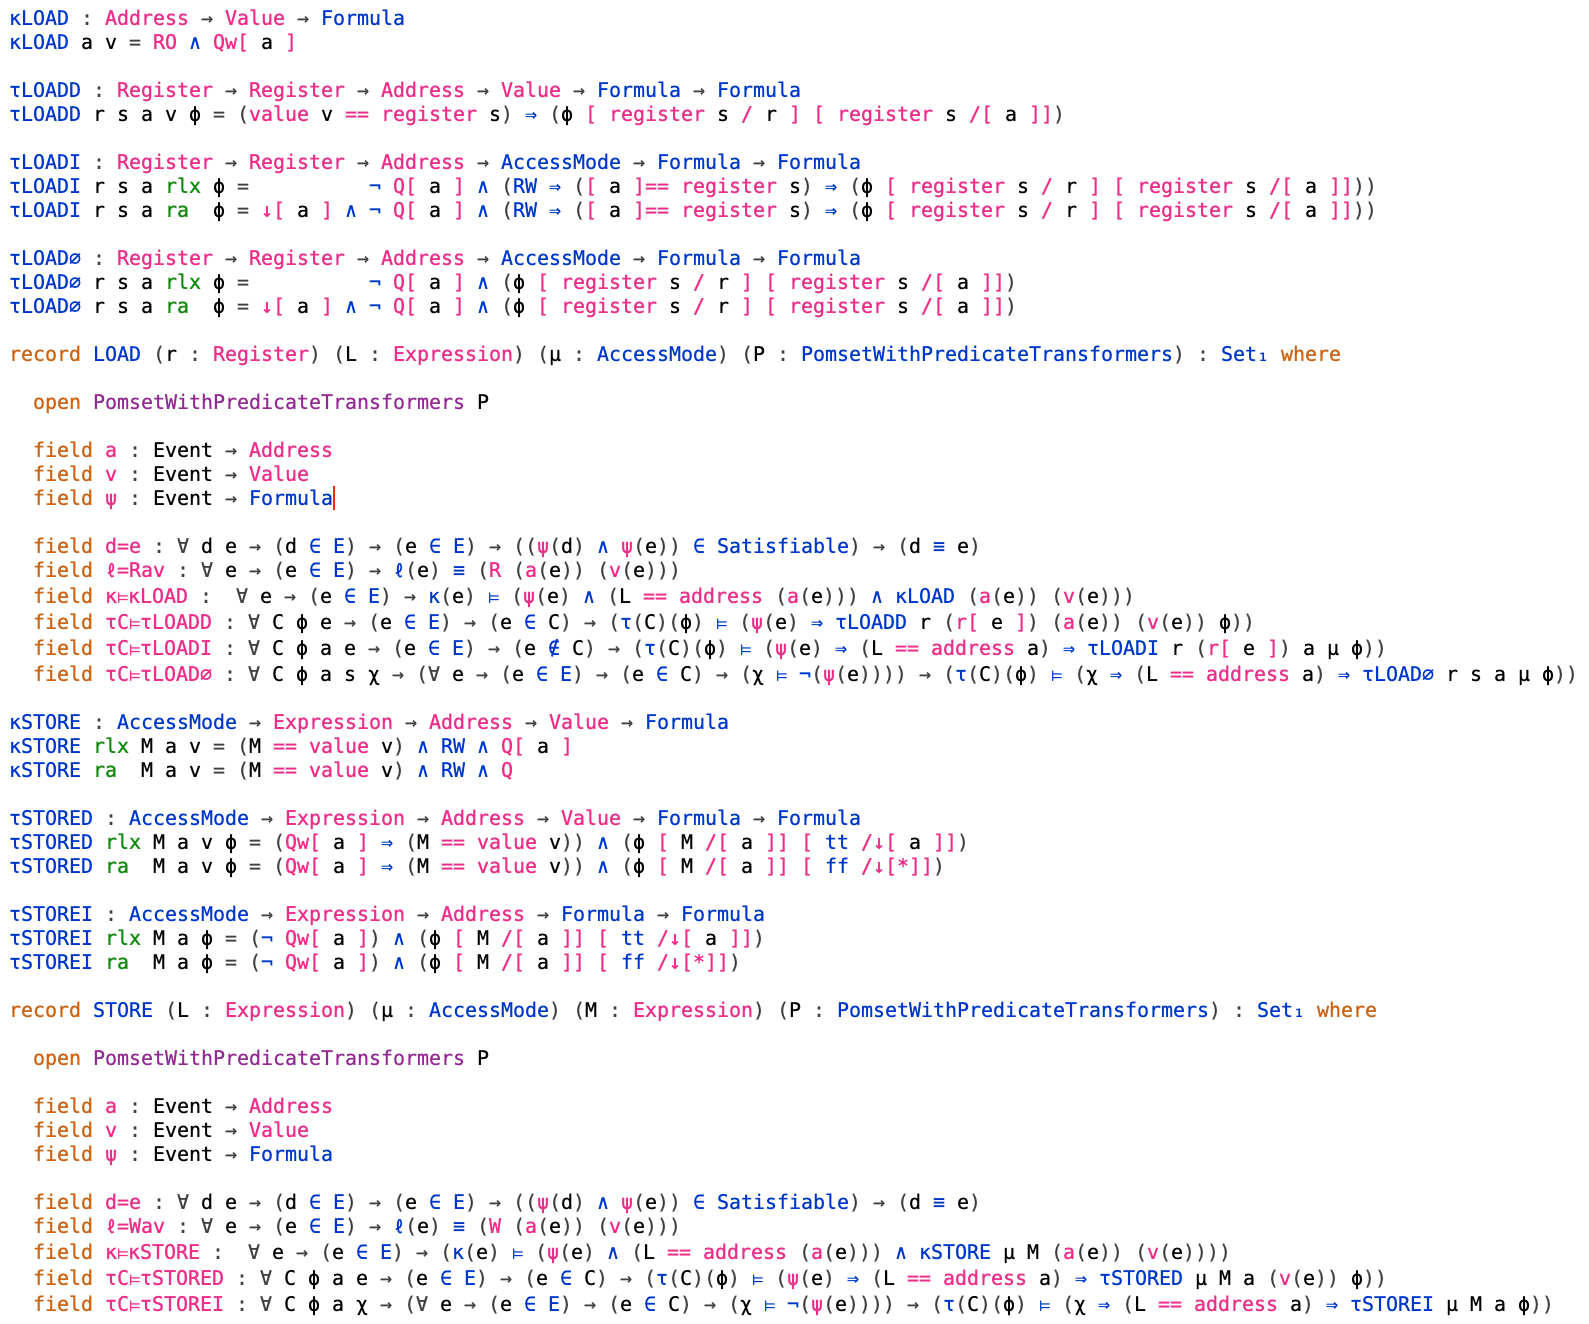
\includegraphics[width=\textwidth]{agda.png}
% \end{figure*}
